\section{Discussion of model}
\label{sec:discussion}
In this section we will make an analysis of the different parts and 
parameters of the model and see what their role in the model is as well 
as inspect their domains and limitations. 


\subsection{Linear approximation}
In our simulation, we use Euler's method to approximate solutions to the equations of motion, 
which are ordinary differential equations, ODE, with initial conditions calculated from last time step, 
and those initial value problems look like:

\begin{eqnarray}
\frac{dy}{dt} &=& f(y),\\
y(t_{0}) &=& y_{0}
\end{eqnarray}

Within some small time interval from $t_{0}$ to $t_{0}+\bigtriangleup t$, the function of $ y(t) $ 
can be approximately represented by a straight line:

\begin{equation}
l(t) = y_{0} + f(y_{0}) (t-t_{0})
\end{equation}

then after a small step size, the function value $ y $ becomes

\begin{equation}
y = y_{0} + f(y_{0}) \bigtriangleup t
\end{equation}

and the calculated value of $ y $ also becomes the initial value for the following step. 
However, this kind of method can cause error in most situations, and there are methods trying 
to minimize the error caused by the numerical way of solving problem.\\

\subsection{The time steps}
\label{sec:timestep}
In this section we discuss how to set the the time steps of the calculation.
When we do the simulations we want it be as cheap as possible. That is we 
want it to be done with as few calculations as possible. Because the cheaper 
you make the simulations the more pedestrians you can have in your simulation 
without waiting to long for the results to come out. One of the way to minimize 
the number of calculations is by choosing the highest possible value for 
$\Delta t$. For instant there would be no reason to make a simulation in a 
time step making people move so little that they, in the same time step in 
real life, would not be able to make a reaction on the changes. On the other 
hand there will of course be a maximum we can choose if we still want the simulations to 
look realistic. If all the pedestrians make big jumps in each time step it will not be very 
good to compare with real life situations. So we have to make sure that people are not able 
to land on top of each other or to pass through a wall because the repulsion forces are 
calculated at to great a distance compared to how big jumps a pedestrian can make.
One of the big challenges when doing simulations is to choose the right value for $\Delta t$. 
One way to get a quantitative value for $\Delta t$ is by looking at at the size of the parameters 
added to the model to get some idea about the maximum displacement of a pedestrian as a function 
of time and then choose a value that seems reasonable.
So the step size also has to be small enough for the simulation and the result to be realistic.
We can see that the error caused by the numerical approach must depends on the step size.
From the mathematical point of view, a smaller step size generally gives smaller error through
Euler's method, since the numerical result gets closer to the actual result, but 
as we use the computer to do the calculation and it only deals with rational numbers, the 
round off error becomes prominent since more calculations are needed.
The round off error from previous steps are being calculated in the next calculations, and when the rounding errors accumulate  
the numerical result of the ODE gets unsatisfactory, since the rounding errors do not decrease at the theoredical rate \cite{RoundingError}.
Arciniega and Allen, 2003 concludes that the rounding error is inversely proportional to the squareroot of the stepsize.
\\
Therefore, an optimal step size could be the one that causes 
the sum of two sources of errors smallest. See figure \ref{timestepfigure} for a sketch of the
idea.



\begin{figure}
    \centering
    {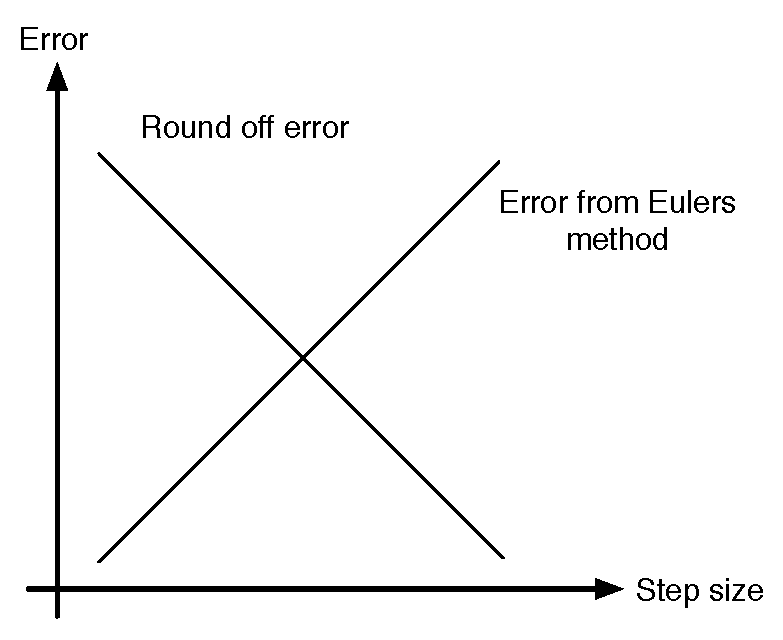
\includegraphics[scale=0.45]{Figures/timestepfigure.pdf}} 
    \caption[Errors from timestep size and Euler's method]{Illustration of how size of the timestep and the round off error interact.
	     The bigger the step size are the greater errors from Eulers method are, but the round off error will get smaller.
	     In contrast the smaller step size are the smaller the errors from Eulers method will be, but the greater the round off
	     errors will get. It follows that there will be a point, step size, where the combined error from Eulers method and round off error
	     will be minimum.}
    \label{timestepfigure}
\end{figure}

\subsection{The fluctuation term}
In addition to all the forces action on the agent the change in velocity of agent 
$\alpha$ is controlled by fluctuation term. The role and nature of this term will 
be discussed in this subsection.

For the acceleration of pedestrian $\alpha$ we have following equation to add up the forces

\begin{equation}
\frac{d\vec{v}_{\alpha}}{dt}=\vec{f}_{\alpha}(t)+\vec{\xi}_{\alpha}(t)
\end{equation}

In this equation, $\vec{f}_{\alpha}(t)$ is the forces acting on pedestrian $\alpha$. 
The term $\vec{\xi}_{\alpha}(t)$ is called a fluctuation term and is added to the equation 
to reflect random behaviour of a pedestrian, in this case $\alpha$. In other words, $\vec{\xi}$ 
adds a stochastic behaviour to the model for each person and because of this, one can't expect 
the same simulation to give the completely same result as a previous simulation with the same 
initial conditions. The reason this term is added is that you would'nt expect every person to 
act with optimal behaviour in all situations. In some way you could also say that $\xi$ is a 
personality factor, taking into account the little differences in the behaviour of different 
persons.

When we choose a value for $\xi$ for each pedestrians, it is of course important that the 
pedestrians in the model will still behave in a way that are realistic. Therefore we do not 
want the fluctuation term to be the dominant factor that makes a person jump 5 meter for no reason. 
Instead it should be the little difference that in some cases makes a pedestrian, $\alpha$, go left 
instead of going right when passing another pedestrian, $\beta$, or something similar.  

When a reasonable mean value for $\xi$ have been chosen a good way to make a value for each 
pedestrian would be with the Gaussian distribution function. This would make the main part of 
the pedestrians have almost the same value but of certain percentage of the pedestrians would 
have greater or lower value representing different personalities like old people or children, 
or people in panic or people that in some other ways have disabilities. 
